\chapter{Supplemental Information}\label{app:supplemental-information}


\section{User Manual}
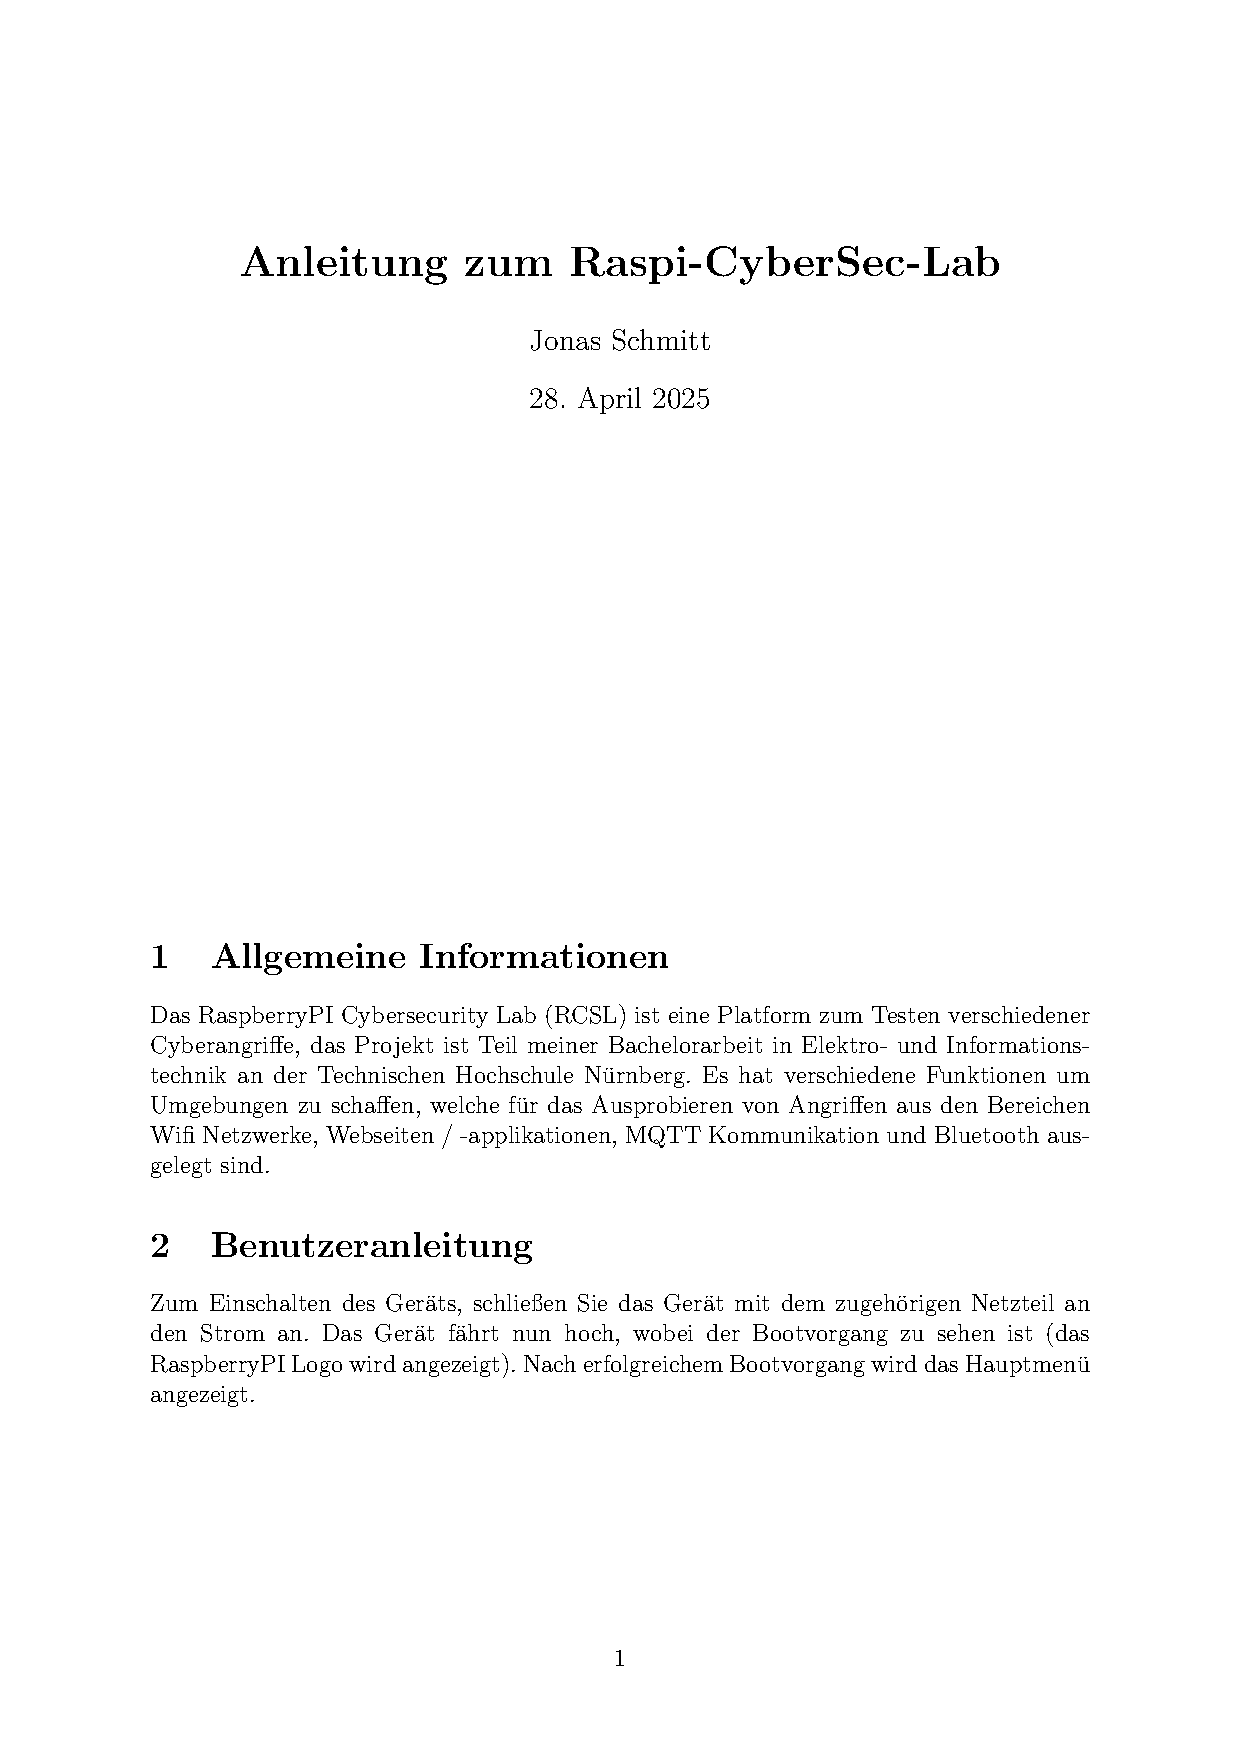
\includepdf[pages={1-}]{userguide/userguide.pdf}

\section{WiFi Basics}

\subsection{Architecture}\label{ssec:A_wifi_architecture}
IBSS networks don't have any APs, instead the STAs are connected directly to each other.
WDS can be used when the reach of an AP needs to be extended, but there is no wired connection available. 
A secondary AP can be installed, which receives backhaul connection from the first AP.
Mesh Networks are complex BSS networks with multiple APs, which the STAs can hop between.
This type of network can improve the signal coverage and resilience and is often used in companies or public institutions. \cite[page~8-9]{Sankaran_Gulasekaran_2021}

\subsection{MAC Frames}\label{ssec:A_wifi_mac_frames}
In a BSS network the frame header is configured for the following functions:

\begin{itemize}
    \item \textbf{Frame Control:} serves different control functions
        \subitem \textbf{Protocol Version:} describes which version of the MAC protocol this frame uses
        \subitem \textbf{Type:} describes the type of MAC frame is being used: there are data, management, control and acknowledgment frames
        \subitem \textbf{Subtype:} describes the subtype of the frame, e.g. association request or beacon frame
        \subitem \textbf{From/to ds:} indicates the direction of travel
        \subitem \textbf{More Fragment:} indicates more following fragments
        \subitem \textbf{Retry:} indicates that the current frame is a retransmission
        \subitem \textbf{Power Management:} gives information about the power state of the STA
        \subitem \textbf{More Data:} indicates more frames are to be transmitted 
        \subitem \textbf{Protected Frame:} indicates whether a frame is encrypted
        \subitem \textbf{Order:} set to 1 if the order of processing is important
    \item \textbf{Duration:} indicates the time of the transmission, therefore how long the medium is occupied
    \item \textbf{Address 1:} contains the receiver address (RA), which can be the MAC address of the destination STA or the BSSID of the AP, depending on the direction, the frame travels
    \item \textbf{Address 2:} contains the transmitter address (TA), which can be the BSSID or the source address.
    \item \textbf{Address 3:} contains either the source or destination address
    \item \textbf{Sequence Control:}
        \subitem \textbf{Fragment Number:} ensures the correct processing sequence of the fragments
        \subitem \textbf{Sequence Number:} number of the frame
\end{itemize} 

\subsection{Wi-Fi Security}\label{ssec:A_wifi_sec}
\begin{table}[h]
    \centering
    \ra{1.5}
    \begin{tabular}{@{}l>{\raggedleft\arraybackslash}p{1.8cm}>{\raggedleft\arraybackslash}p{2.4cm}>{\raggedleft\arraybackslash}p{2.8cm}>{\raggedleft\arraybackslash}p{2.7cm}@{}}
        \toprule
        & {WEP} & {WPA} & {WPA2} & {WPA3} \\
        \midrule
        \textit{Certification start} & - & 2003 & 2004 & 2018 \\
        \textit{Mandatory since} & - & 2006 & 2006 & 2019 \\
        \textit{Underlying standard(s)} & 802.11 & 802.11i(part. compliance) & 802.11i, 802.11w(PMF) & 802.11s(SAE), 802.11w\\
        \textit{Information element} & None & WPA IE & RSN IE & RSN IE \\
        \textit{Encryption} & RC4 & TKIP & TKIP, AES-CCMP & AES-CCMP, AES-GCMP \\
        \textit{Authentication} & None & PSK, 802.1X & PSK, 802.1X & SAE, 802.1X \\
        \textit{Usability enhancement} & None & None & WPS & DPP \\
        \textit{Open Wi-Fi security} & None & None & None & OWE \\
        \bottomrule
    \end{tabular}
    \caption{Evolution of Wi-Fi Security \cite[page~123]{Sankaran_Gulasekaran_2021}}
    \label{tab:wifi_security}
\end{table}

\newpage
\section{Documentation}
\subsection{Hardware}\label{ssec:A_docu_hardware}
\begin{figure}[h]
    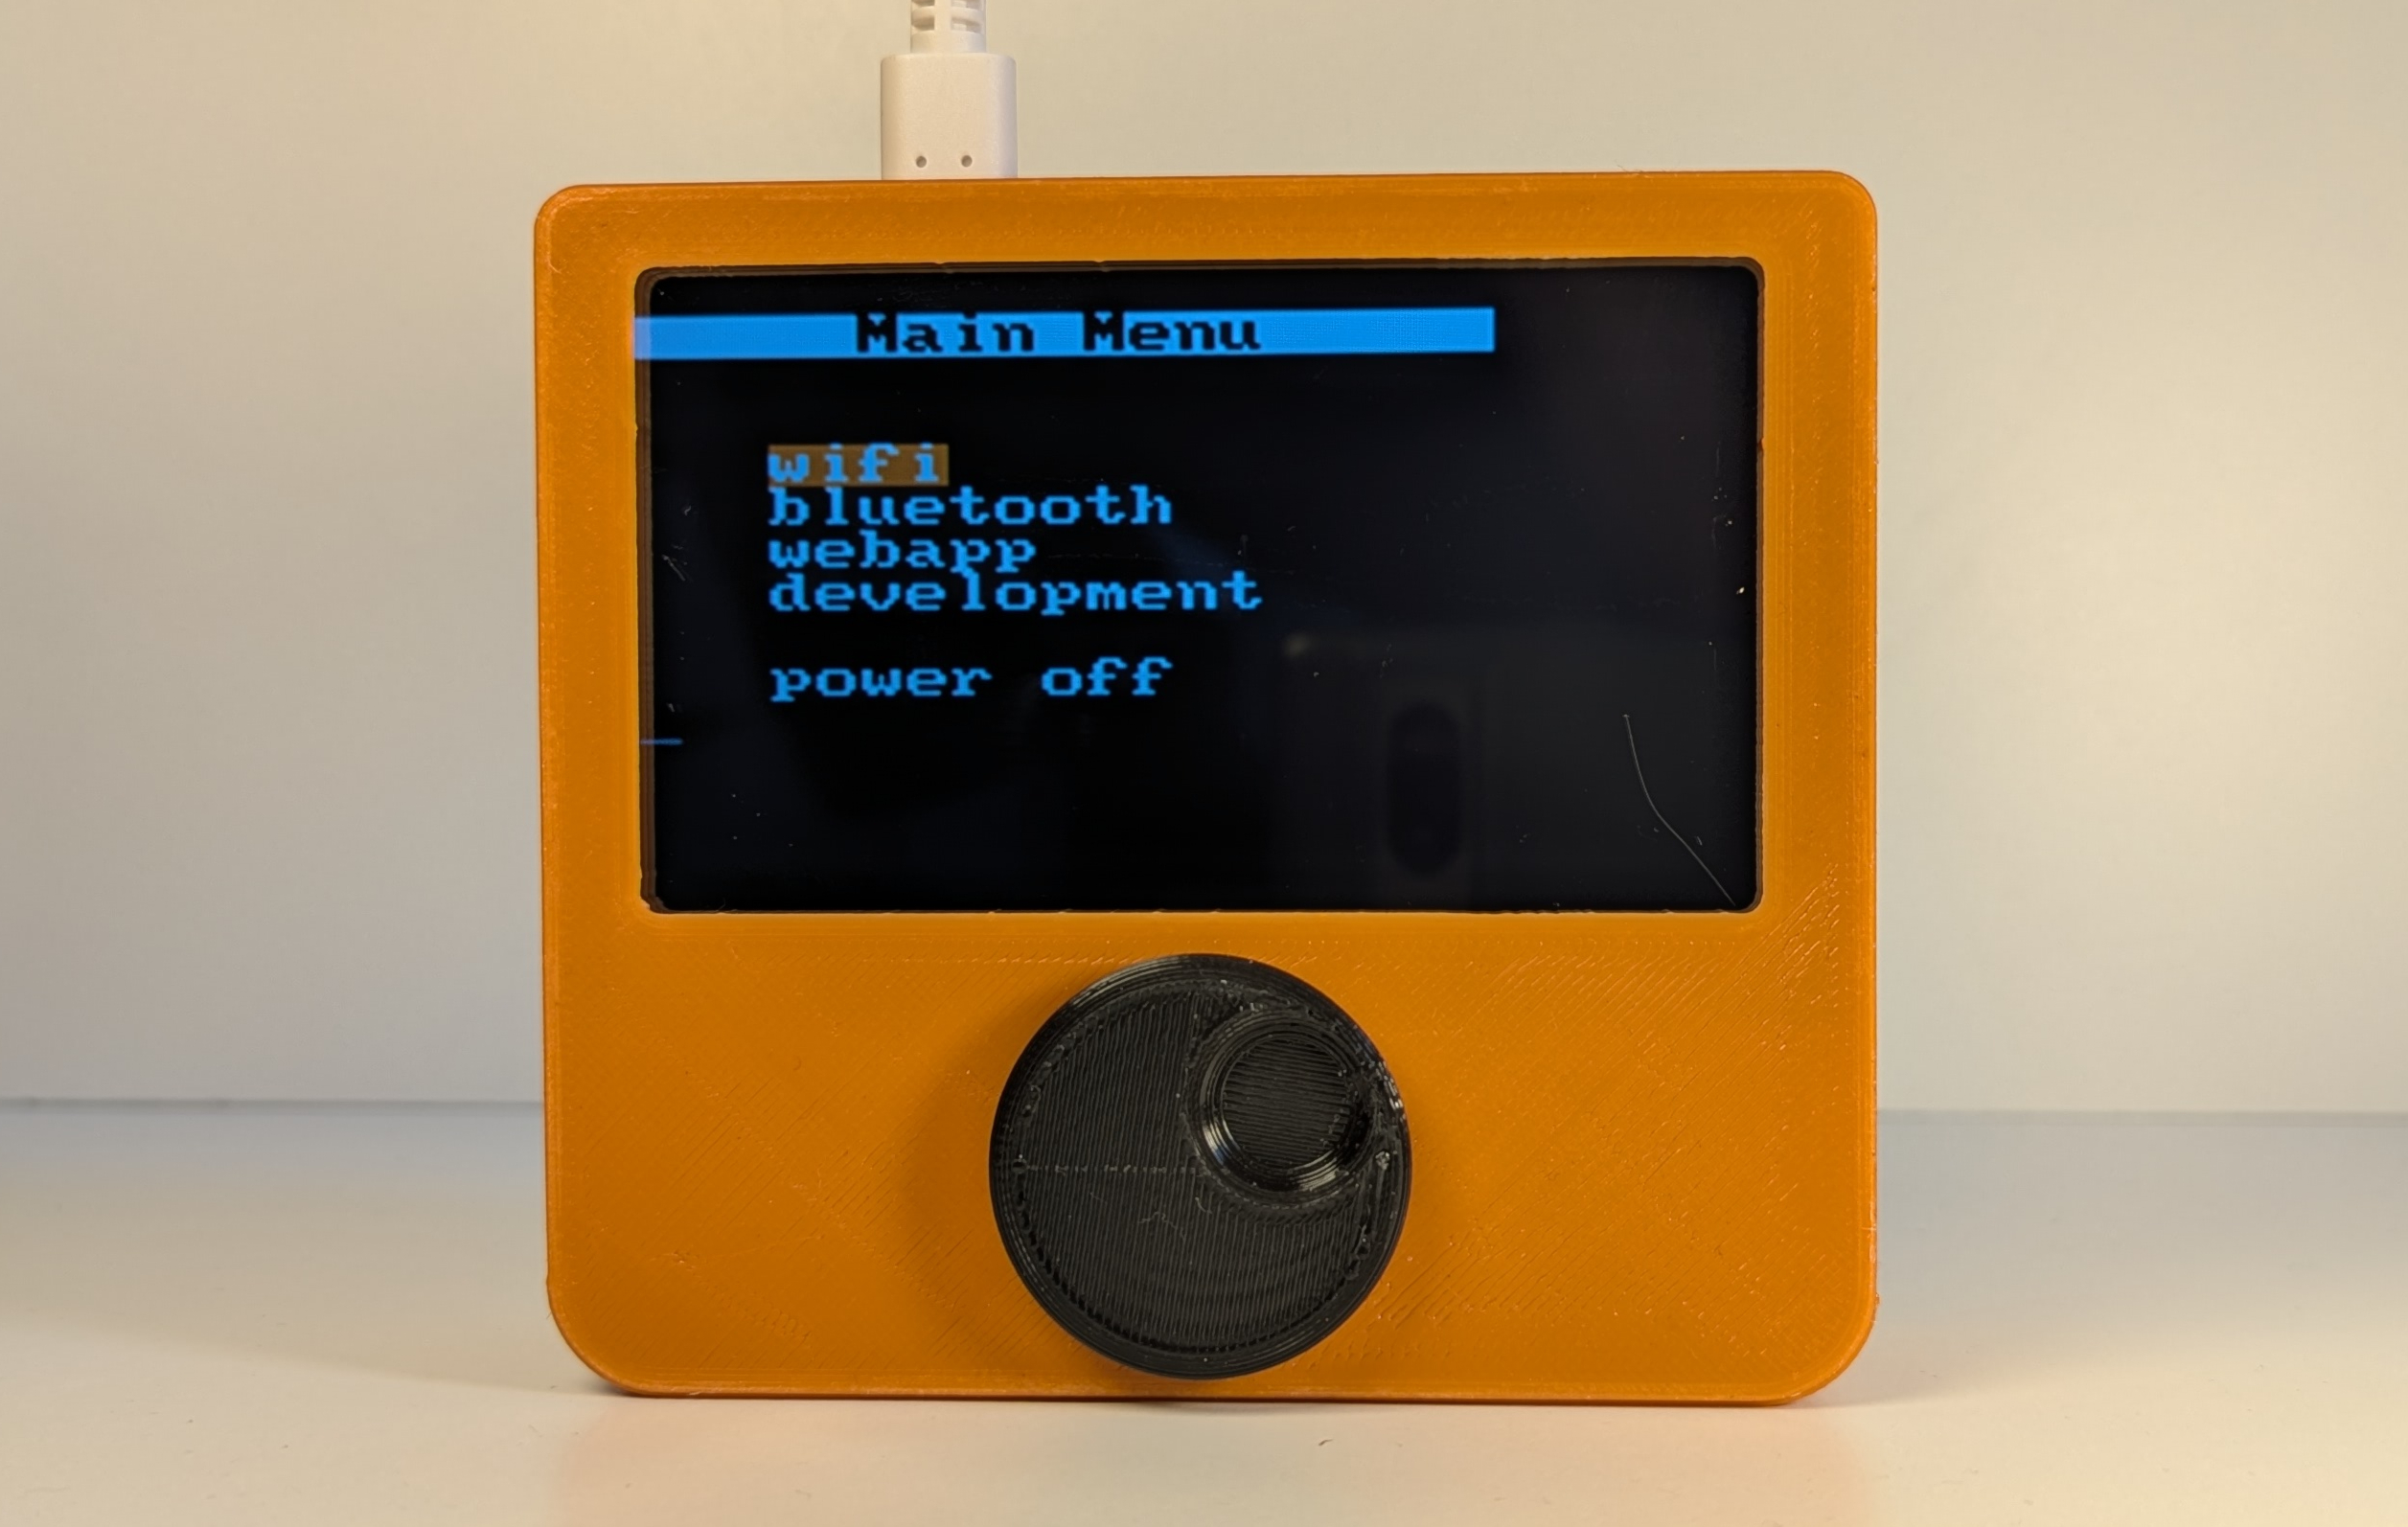
\includegraphics[width=0.9\linewidth]{figures/Abbildungen/Photo_front.jpg}
    \centering
    \caption{RCSL front}
    \label{fig:RCSL_front}
\end{figure}

\begin{figure}[h]
    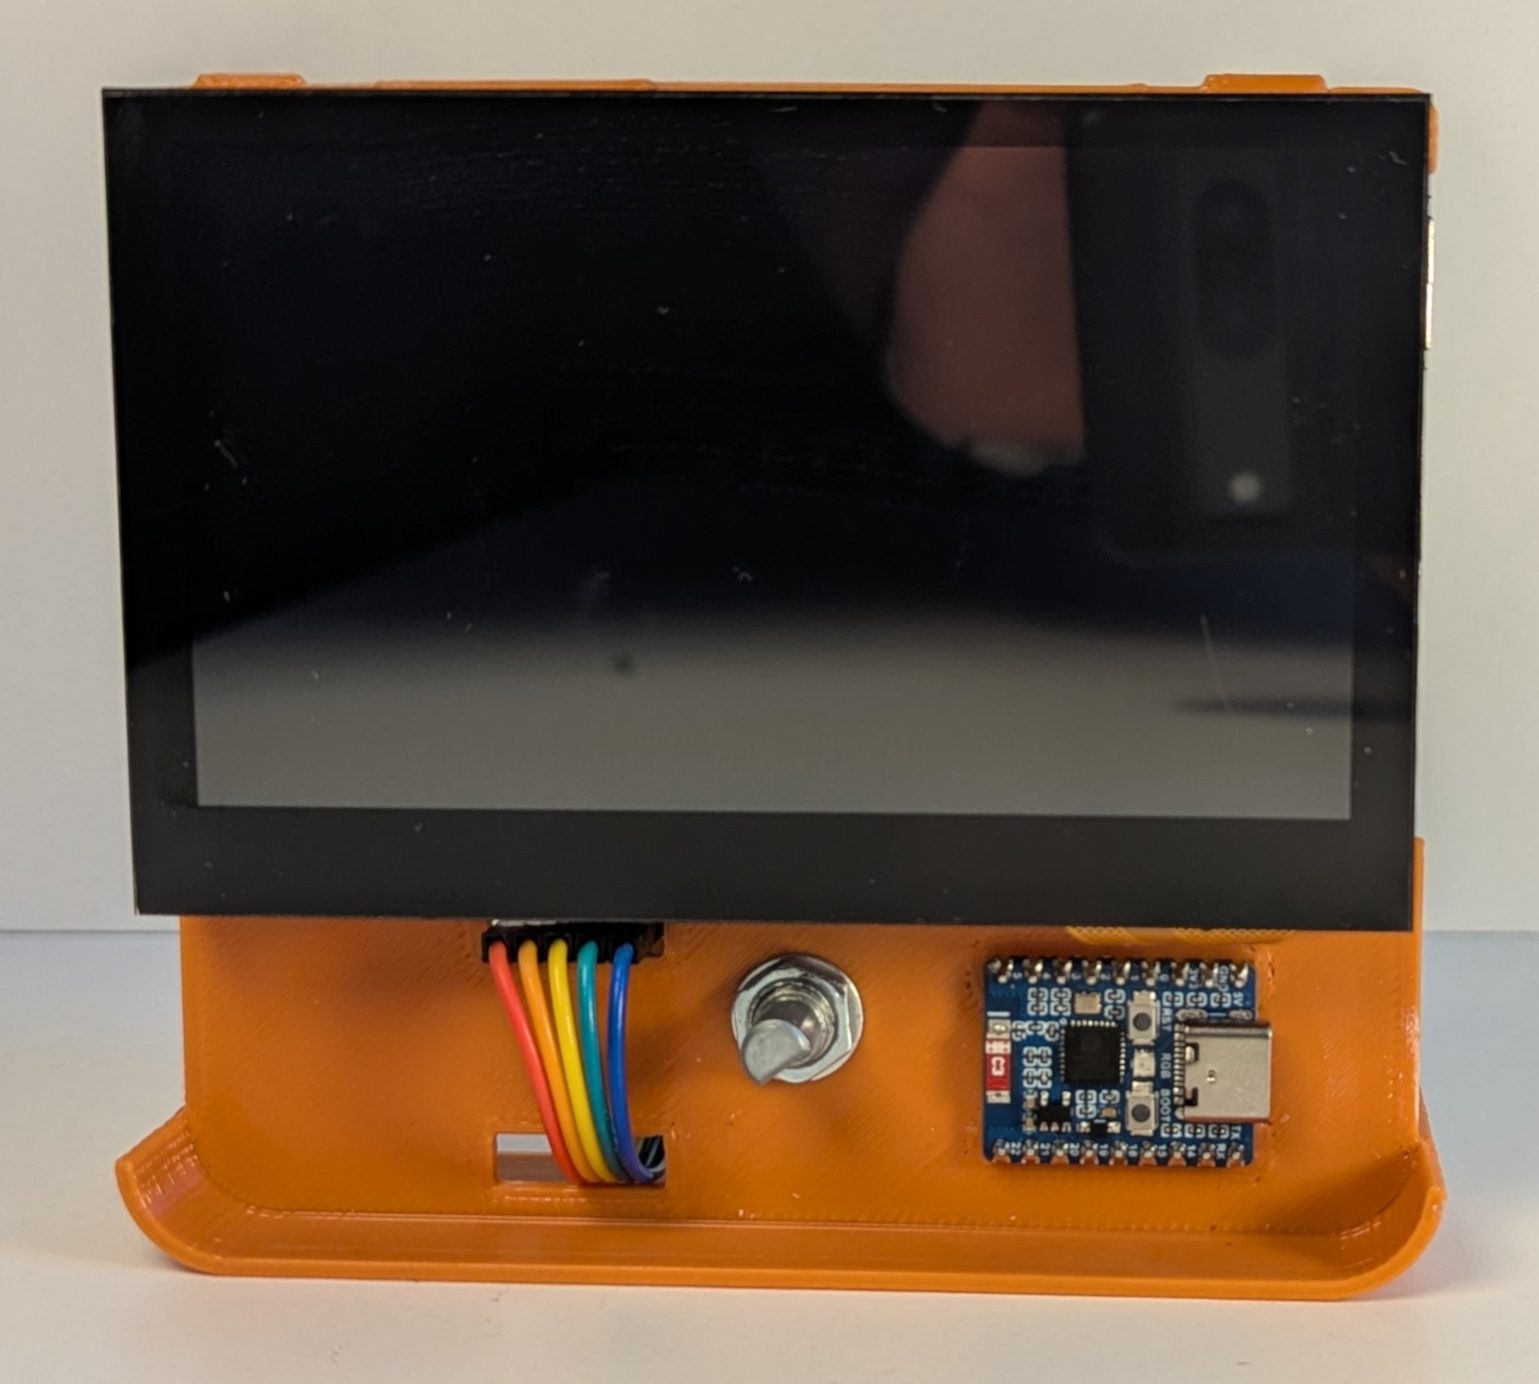
\includegraphics[width=0.45\linewidth]{figures/Abbildungen/Photo_open_front.jpg}
    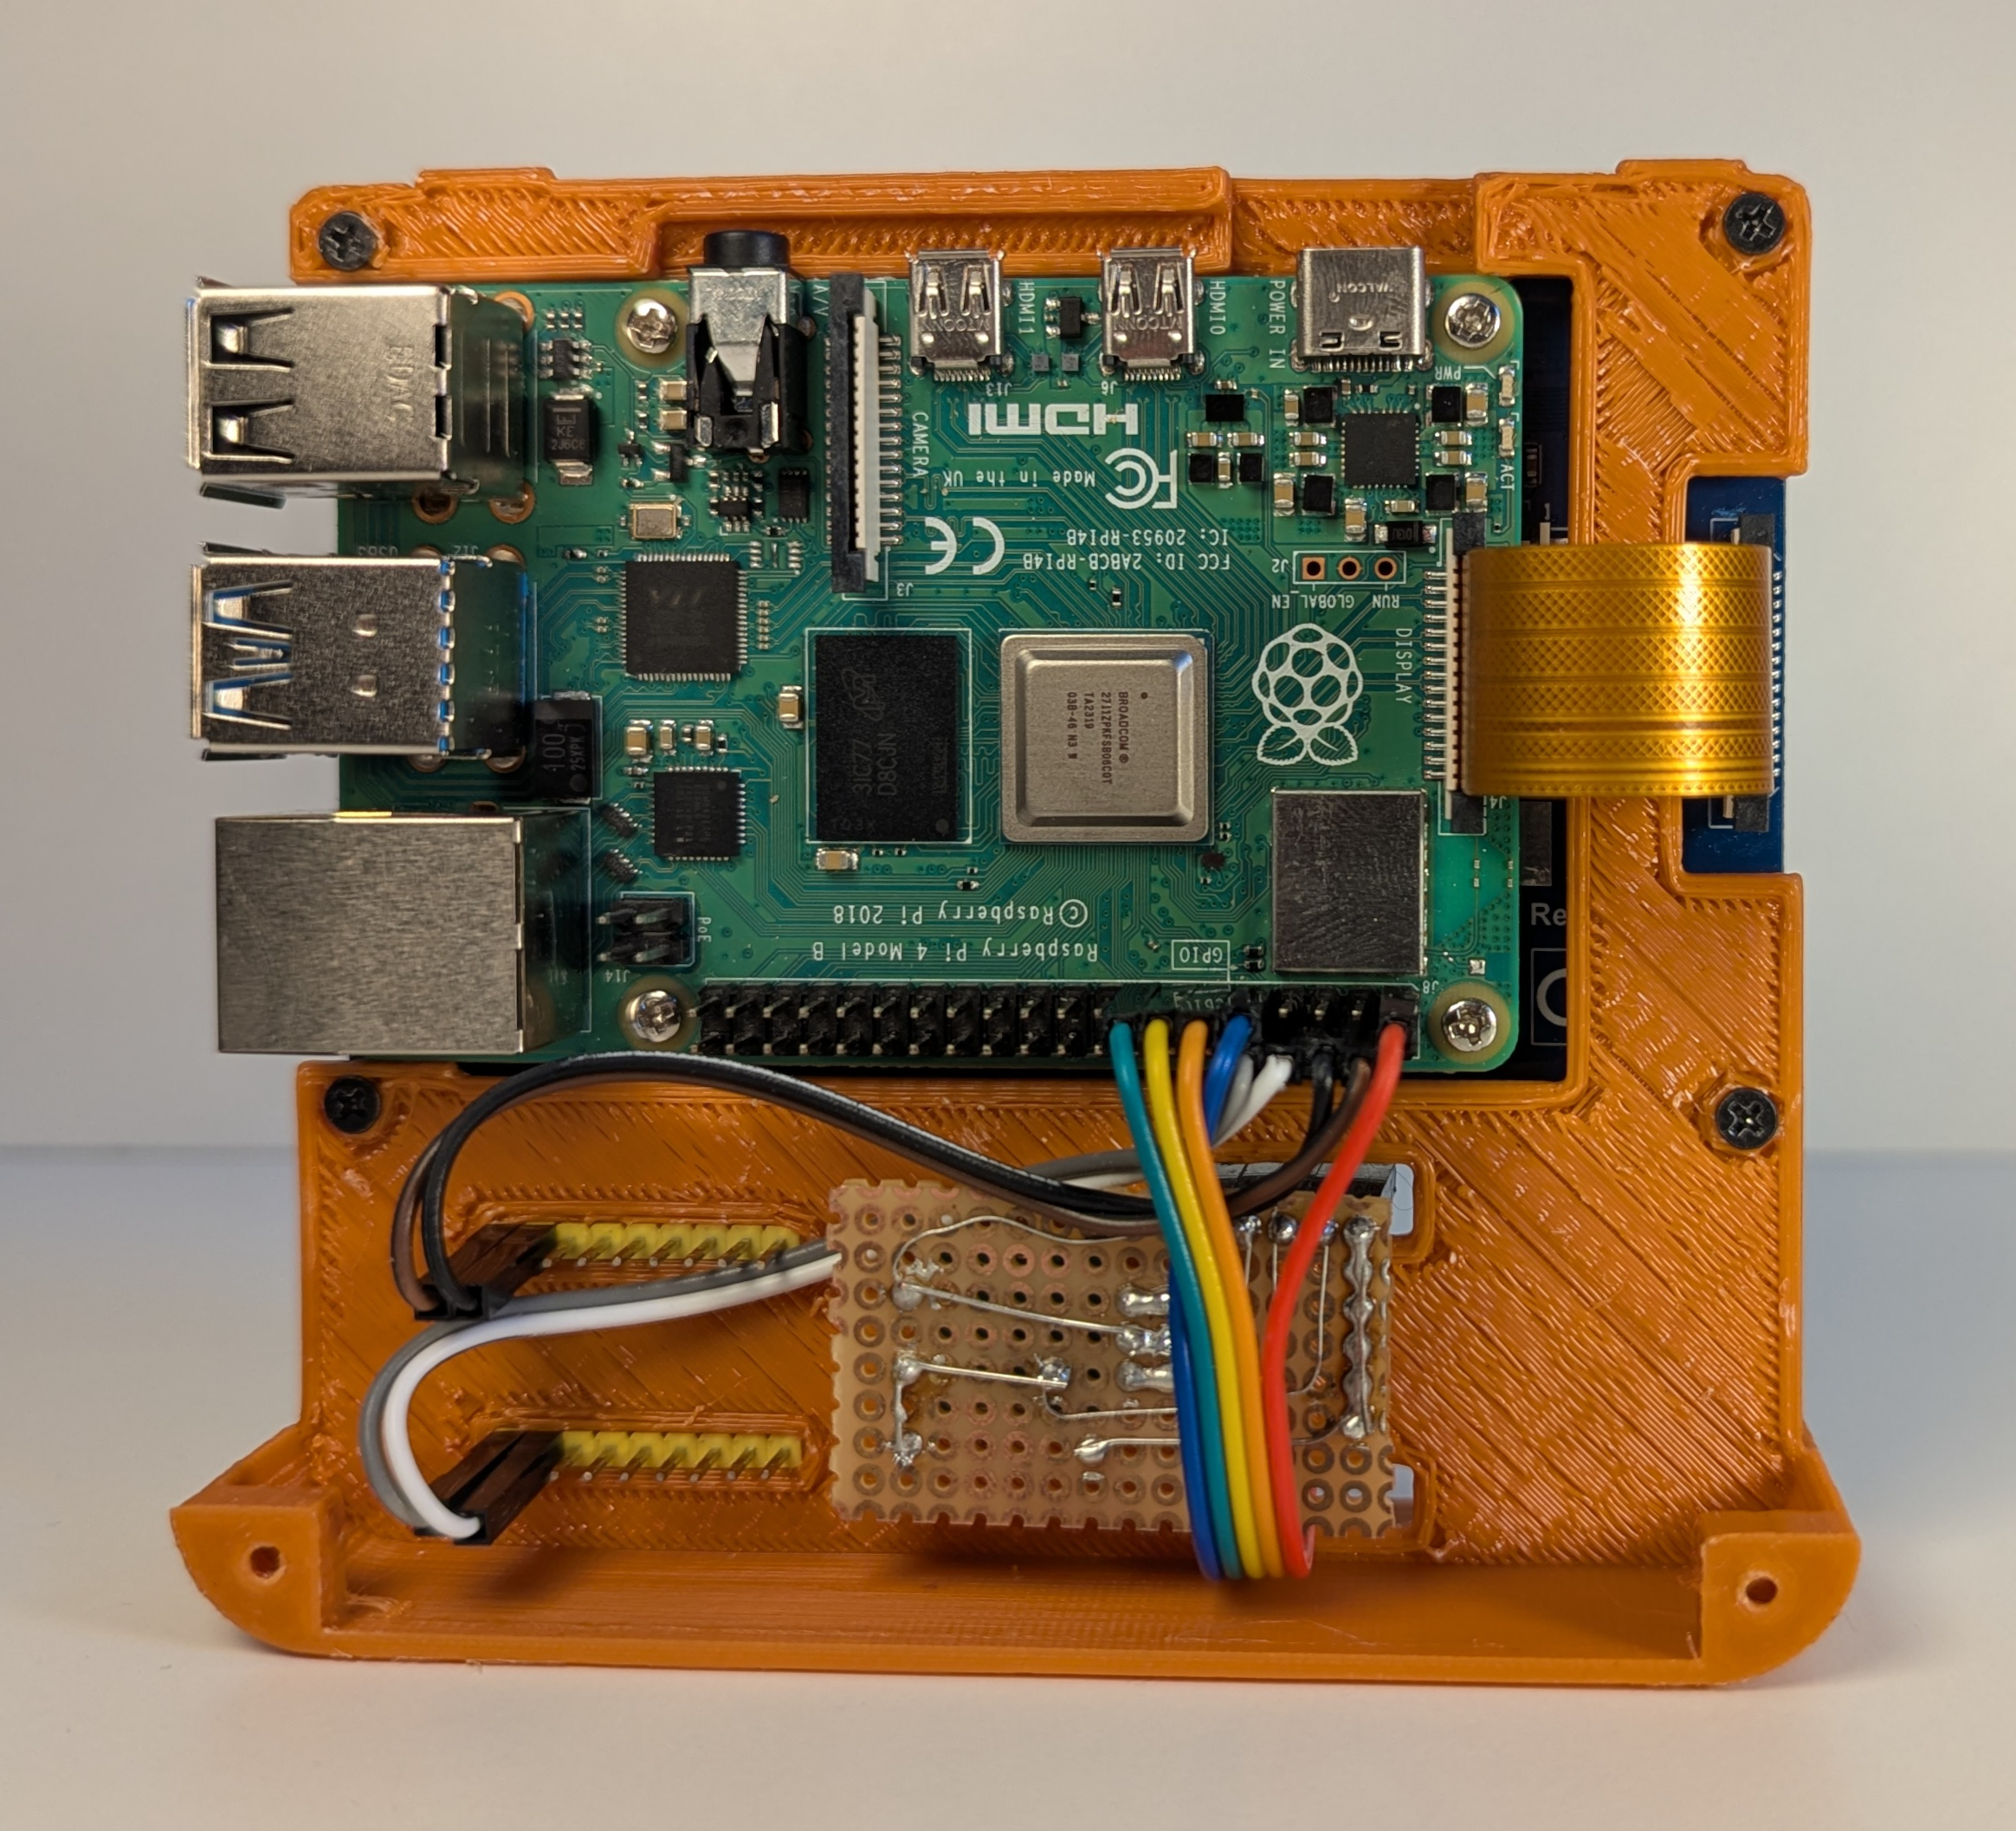
\includegraphics[width=0.45\linewidth]{figures/Abbildungen/Photo_open_back.jpg}
    \centering
    \caption{RCSL without case}
    \label{fig:RCSL_nocase}
\end{figure}

\newpage
\subsection{Software}\label{ssec:A_docu_software}
%\begin{table}[h]
%    \caption{menu and option overview}
%    \label{tab:menus_options}
%    \centering
%    \ra{1.3}
%    \small
%        \begin{tabular}{@{}lrclclrclcl@{}}\toprule
%            \multicolumn{11}{c}{Main Menu} \\
%            \midrule
%            \multicolumn{2}{c}{wifi} && \multicolumn{1}{c}{bluetooth} && \multicolumn{2}{c}{webapp} && development && power off \\
%            \cmidrule{1-2} \cmidrule{4-4} \cmidrule{6-7} \cmidrule{9-9} 
%            activate & WEP && \textit{under} && Juice Shop & on && option 1 && \\
%            & WPA && \textit{development} &&& off && option 2\\
%            & WPA2 &&&& MQTT & on && option 3\\
%            & WPA3 &&&&& off && option 4\\
%            deactivate &&&&&&&& option 5\\
%            status\\
%            new password & WEP\\
%            & WPA\\
%            & WPA2\\
%            & WPA3\\
%            monitor & on\\
%            & off\\
%            & show log\\
%            & delete log\\
%            \bottomrule
%        \end{tabular}
%\end{table}
\centering{\textbf{Menus Overview}}
\begin{itemize}
    \setlength\itemsep{0.1cm}
    \item \textbf{wifi:} options for wifi
        \begin{itemize}
            \item \textbf{activate:} open up a hotspot - runs wifiActivate.sh
                \subitem \textbf{choose the wifi standard}
            \item \textbf{deactivate:} turn off the active network - runs wifiReset.sh
            \item \textbf{status:} display the current networks settings - runs wifiStatus.sh
            \item \textbf{change password:} set new password for a network - runs wifiNewPassword.sh
                \subitem \textbf{choose the wifi standard}
            \item \textbf{monitoring:} settings for wifi monitor - runs wifiMonitor.sh
                \subitem \textbf{on/off/show log/delete log} 
        \end{itemize}
    \item \textbf{webapp:} options for webapps
        \begin{itemize}
            \item \textbf{Juice Shop:} settings for the Juice Shop - runs juiceShop.sh
                \subitem \textbf{on/off}
            \item \textbf{MQTT:} settings for MQTT communication - runs mqtt.sh and the mqtt program
                \subitem \textbf{on/off}
        \end{itemize}
    \item \textbf{development:} runs development options from development.sh
    \item \textbf{power off:} power off the system - runs shutdown.sh
\end{itemize}

\begin{figure}[h]
    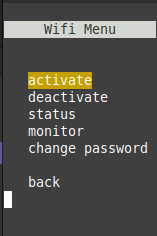
\includegraphics[width=0.25\linewidth]{figures/Abbildungen/hackerypi/menu_wifi.png}
    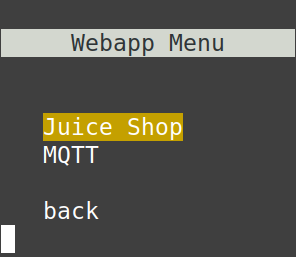
\includegraphics[width=0.3\linewidth]{figures/Abbildungen/hackerypi/menu_webapp.png}
    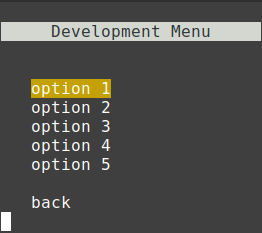
\includegraphics[width=0.35\linewidth]{figures/Abbildungen/hackerypi/menu_dev.png}
    \centering
    \caption{Device menus}
    \label{fig:menus}
\end{figure}

\newpage
\section{Pentesting}

\begin{figure}[h]
    \centering
    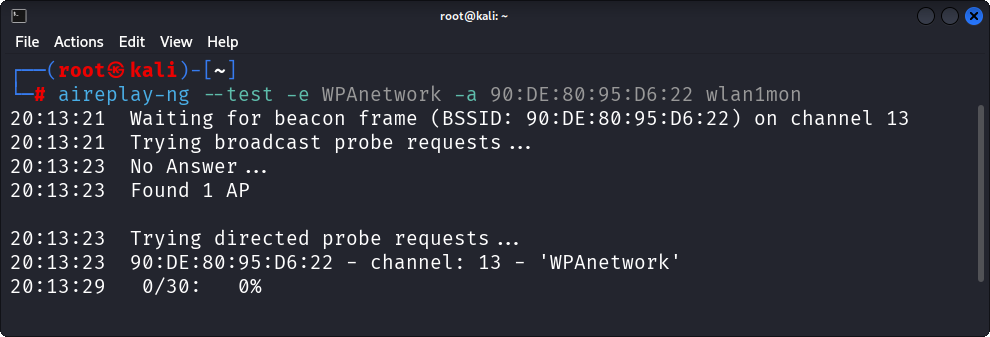
\includegraphics[width=\textwidth]{figures/Abbildungen/Screenshots/aireplay_test_WPA.png}
    \caption{Screenshot of testing frame injection}
    \label{fig:aireplay_test_WPA}
\end{figure}

\begin{figure}[h]
    \centering
    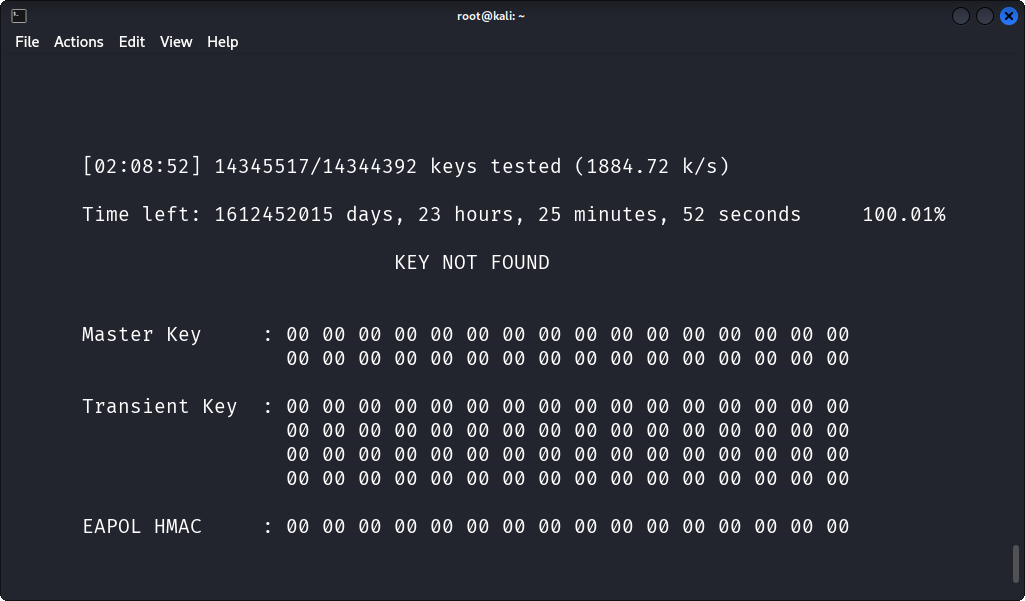
\includegraphics[width=\textwidth]{figures/Abbildungen/Screenshots/aircrack_WPA_fail.png}
    \caption{Screenshot of the failed attempt to crack WPA}
    \label{fig:aircrack-ng_WPA_fail}
\end{figure}